\chapter{Controller Architecture}
\label{controller_architecture}
% /////////////////////// /////////////////////////////

In this chapter, we consider a hierarchical control architecture. First, each vehicle has an embedded High-Level Controller (HLC). It has access to the internet and different kind of services. Here, the goal is to manage the position of the vehicle on the highway, its velocity, and the lane position it should use. Then using the previous information, a Mid-Level Controller (MLC) takes as a reference and moves the vehicle avoiding obstacles that could appear in automated driving. Finally, a Low-Level controller (LLC) is implemented to generate the fair inputs of the vehicle's actuators. It will calculate the power units required to move the vehicle to the desired position. This control layer is simple, and we will not focus on it. Figure \ref{fig:control_architecture} shows the complete architecture. 

\begin{figure}[H]
    \centering
    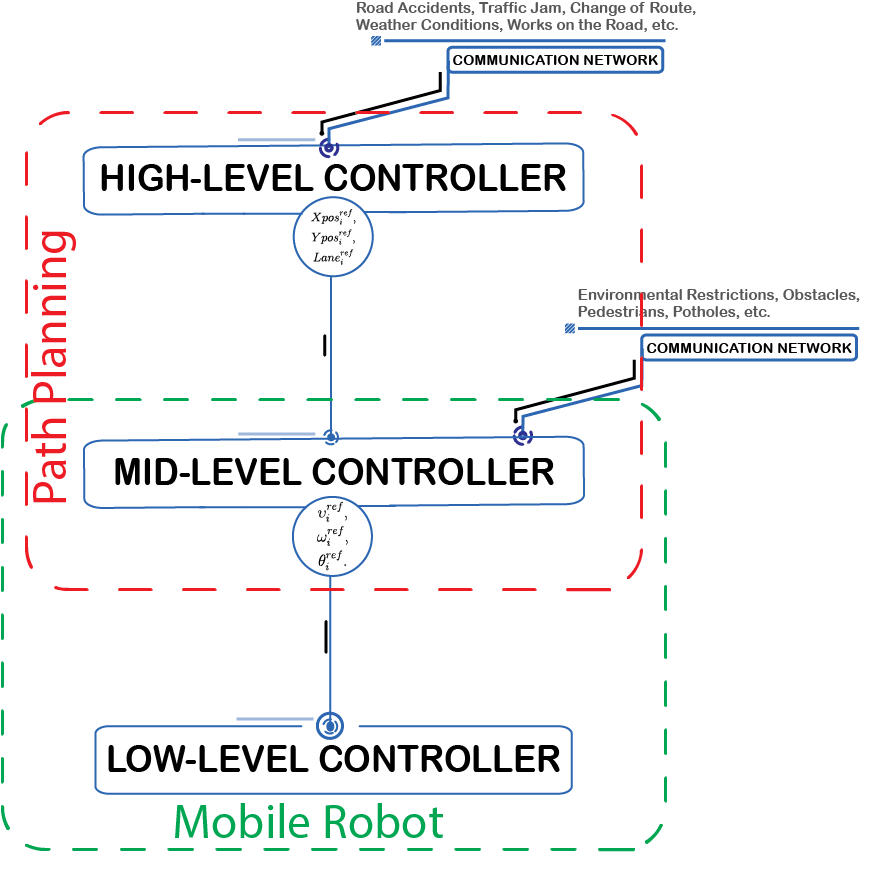
\includegraphics[width=1\textwidth]{Kap4/architecture.png}
    \caption{Control architecture}
    \label{fig:control_architecture}
\end{figure}

% /////////////////////// reference generator/////////////////////////////

\subsection{High-Level Controller: GMIPG}
A Model Predictive Control (MPC) with a Generalized Mixed-Integer Potential Game ( GMIPG) framework was designed and implemented for high-level control to guarantee that the vehicles follow the basic traffic rules. MPC is helpful because it could prevent future issues and pre-correcting signal inputs from achieving the main objective. The GMIPG is necessary to control the vehicle in specific parameters. Each vehicle has to be in an integer number of the lane (1,2,3,..., N) and use binary variables to activate some logical constraints; therefore, we implement the Mixed Integer variables. Furthermore, finally, it is a multi-agent game where each agent aims for a selfish objective. We use a generalized potential game structure to achieve a global and fair solution. 


Each vehicle has a solid and large number of variables of control and sense. The HLC uses a set of network variables such as velocity, acceleration, lane position, and future states. Some of them are part of the information shared by the other agents, and the users give the other one. However, we assume that:
\begin{itemize}
    \item Each road user aims to pursue their selfish objective.
    \item Each control system has a full connection to the entire network.
    \item The communication does not have lags or problems in sharing the desired information.
    \item The selfish objective of each vehicle could be a result of a personal decision o a result of an intelligent algorithm., e.g., maps, Waze, or some traffic and routing algorithm.
    \item Crossroads, traffic lights, or intersections are not part of the experimental environment.
\end{itemize}

This thesis document aims to manage, control and guarantee safe automated driving in the most common situation a vehicle can face on a highway against agents who make selfish decisions. Specially, we focus on the mixed-integer decision-maker layer for motion planning of the vehicles.

% ////////////////////////////////////////////////////////////////////////////

\subsection{Mixed-Integer Linear Constraints}

Chapter \ref{linear_model_system} explains the autonomous driving rules to make driving safe without affecting the objective of each agent. In this section, we will convert the above rules into linear logical constraints. Due to the previous, the control algorithm can constrain the solution space to one that is safe for the environment. Two different types of constraints will be discussed: lateral and longitudinal.



\\

\begin{equation}
\left\{ \begin{matrix}
\begin{aligned}
\min_{v,a,z, l_i^l,l_i^r} \quad & J_i\left ( v_i, a_i, z_i \right )\\
\textrm{s.t.} \quad & v_i(t+1) = v_i(t)+\tau a_i(t),\\
  &   z_i(t+1) = z_i(t) + l_i^l(t) - l_i^r(t),   \\
& a_i(t) \in \mathcal{A} ,  \\
& v_i(t) \in \mathcal{V_i} ,  \\
& a_i(z) \in \mathcal{L_i} ,  \\
&  l_i^l(t),l_i^r(t)\in \mathbb{B},   \\
& l_i^l(t) + l_i^r(t)  \leq 1.\\
\end{aligned}
\end{matrix}\right.

\end{equation}

\\


% \begin{equation}
%     \mathcal{V}_i(t) := [0,\overline{v_i}] \cap[v_i(t)+\tau \underline{a_i}, v_i(t)+\tau \overline{a_i} ],\\
% \end{equation}
   
% \\


% \begin{equation}
% \mathcal{L}_i(t) := \mathcal{L} \cap[z_i(t)-l_i^r, z_i(t)+l_i^l].
% \end{equation}



% \subsection{}
% ////////////////////////////////////////////////////////////////////////////
\subsubsection{Longitudinal Constraints}


% ////////////////////////////////////////////////////////////////////////////


% \subsubsection{Preliminaries}
Let us consider the safety rules in Section \ref{linear_model_system} where it should be fulfilled that if a pair of vehicles circulated in the same lane and with a distance greater than zero, a safety distance should be observed: 


\begin{equation}
    %  \label{eq:4_6}
 [z_{i,j}(t)=0] \wedge [\left | d_{ij}(t) \right | \geq 0] \Rightarrow [\left | d_{ij}(t) \right | \geq D_i^s]
%  \label{eq:4_7}
\end{equation}

We introduce two logical and binary variables, $\alpha ,\beta \in \mathbb{B} := \left\{ 0,1 \right\}$. The variable $\alpha$ discriminates between vehicles travelling in the same lane at the same time $(l_{i,j}=0)$, and $\beta$ discriminates between vehicles ahead $(\beta=1)$ or behind $(\beta=0)$, no matter what lane they are on

\begin{align}
 [\alpha_{i,j}(t) = 1] & \Leftrightarrow [z_{i,j}(t) \leq 0] \wedge [z_{i,j}(t) \geq 0]
 \label{eq:4_3}
 \\
 [\beta_{i,j}(t) = 1] & \Leftrightarrow  [d_{i,j}(t) \geq 0]
 \label{eq:4_4}
\end{align}



Therefore, the equations \ref{eq:4_3} and \ref{eq:4_4} can be written as nonlinear inequalities:

\begin{equation}
    \alpha _{i,j}(t)[\beta_{i,j}(t)(d^s_i(t)-d_{i,j}(t)) + (1-\beta_{i,j}(t))(d^s_i(t)+d_{i,j}(t) )] \leq 0,
    \label{eq:4_5}
\end{equation}

Relying on the pattern of inequalities summarized in Table \ref{Table_1}, we will use it to handle the logical implications and nonlinear constraints. Therefore, let us consider the right-hand side of the equation \ref{eq:4_3}. Introducing $\eta$ and $\theta \in \mathbb{B}$, where if $z_{i,j} \leq 0$  implies $\eta_{i,j} = 1$  :

\begin{equation*}
    [\eta_{i,j}(t) = 1] & \Leftrightarrow [z_{i,j}(t) \leq 0]
\end{equation*}

and is translates into $\mathcal{S}_\leq (\eta _{i,j}(t),z_{i,j}(t),0)$. The same way if $\theta_{i,j}=1$ implies $z_{i,j} \geq 0$ :

\begin{equation*}
    [\theta_{i,j}(t) = 1] & \Leftrightarrow [z_{i,j}(t) \geq 0]
\end{equation*}

and is translates into $\mathcal{S}_\geq (\theta _{i,j}(t),z_{i,j}(t),0)$. 
Finally the equation \ref{eq:4_3} is represented as follows:

\begin{equation}
 (\textbf{\ref{eq:4_3}}) \Rightarrow \left\{\begin{matrix}
\mathcal{S}_\leq (\eta _{i,j}(t),z_{i,j}(t),0),\\ 
\mathcal{S}_\geq (\theta _{i,j}(t),z_{i,j}(t),0),\\ 
\mathcal{S}_\wedge (\alpha_{i,j}(t),\eta _{i,j}(t), \theta_{i,j}(t)).
\end{matrix}\right. 
\label{eq:4_6real}
\end{equation}

The same procedure is used to transform the equation
\ref{eq:4_4} in a mixed-integer linear constraint:

\begin{equation}
    (\textbf{\ref{eq:4_4}}) \Rightarrow \mathcal{S}_\geq (\beta_{i,j}(t),d_{i,j}(t),0).
\end{equation}

Now let me factor the equation \ref{eq:4_5} into a reduced non-linear equation.

\begin{equation}
-2 \ \underbrace{\alpha_{i,j}(t) \beta_{i,j}(t)}_{\xi_{i,j}(t)} \ d_{i,j}(t) + \alpha_{i,j}(t) \ 
 d^s_{i}(t) + \alpha \ d_{i,j}(t) \leq 0.
    \label{eq:4}
\end{equation}

As we can see, the equation is nonlinear and is composed of binary and integer variables. In the equation \ref{eq:4} we transform $\alpha_{i,j}(t) \beta_{i,j}(t)$ into $\xi_{i,j}(t)$ in order to linearize the equation. 
\\
\begin{equation*}
    \mathcal{S}_\wedge (\xi_{i,j}(t),\alpha_{i,j}(t),\beta_{i,j}(t)).
\end{equation*}

The next and last step to linearize the equation is to transform the multiplication of a binary variable and integer variable into real auxiliary variables. We define $f_{i,j}(t) := \xi_{i,j}(t) d_{i,j}(t) $ , $g_{i,j}(t) := \alpha_{i,j}(t) d^s_i(t)$ , and $h_{i,j}(t) := \alpha_{i,j}(t) ,d_{i,j}(t)$ that shall satisfy $\mathcal{S}_\Rightarrow$ in the Table \ref{Table_1} as follows:

\begin{align}
\mathcal{S}_\Rightarrow & (f_{i,j}(t),d_{i,j}(t),\xi_{i,j}(t)).
\\
\mathcal{S}_\Rightarrow & (g_{i,j}(t),d^s_i(t),\alpha_{i,j}(t)).
\\
\mathcal{S}_\Rightarrow & (h_{i,j}(t),d_{i,j}(t),\alpha_{i,j}(t)).
\end{align}

Finally, the equation \ref{eq:4_5} is expressed as a linear mixed integer constraint equation:

\begin{equation}
    -2f_{i,j}(t)+g_{i,j}(t)+h_{i,j}(t) \leq 0.
\end{equation}




% ///////////////////////////////////////////////
\subsubsection{Lateral Constraints}
Let us consider the scenario in Figure \ref{fig:lat_col} where two vehicles are side by side. The second Mixed-Integer coupling constraint we introduce is about avoiding collision between vehicles driving next to each other on a highway. It was explained in the Algorithm \ref{alg:lat_saf} in section \ref{linear_model_system} how each agent's restrictions must have to avoid a lateral collision. Therefore, we implement the same transformation as in the previous section. The main idea is to linearize a logical constraint equation into a set of Mixed-Integer Linear Constraints that can avoid lateral vehicles regardless of the situation. The Algorithm \ref{alg:lat_saf} can be transformed first as a logical implication form 


\begin{equation}
[\left |z_{i,j}(t)  \right |=1] \wedge [\left | d_{ij}(t) \right | \leq \hat{d}] \wedge \left \{ [l_i^r(t)=1] \vee[l_i^l(t)=1] \right \}\Rightarrow [z_{i,j}(t+1)-z_{i,j}(t)=0].
\label{eq:4_8}
\end{equation}

\\
It represents the behaviour that each agent should have in a collision risk situation. However, the logical constraints model cannot be solved by MPC due to non-linearities and non-convexity. Therefore, we transform the previous equation into multiple linear inequalities that will allow the controller to find an optimal answer. As in the previous transformations, let us consider three auxiliary variables $\gamma^l$, $\gamma^r$ and $\zeta \in \mathbb{B}:$


\begin{align*}
[\gamma^l _{i,j}(t) = 1] \Leftrightarrow & [z_{i,j}(t) \leq 1] \wedge [z_{i,j}(t) \geq 1]
\\
[\gamma^r_{i,j}(t) = 1] \Leftrightarrow & [z_{i,j}(t) \leq -1] \wedge [z_{i,j}(t) \geq -1]
\\
[\zeta_{i,j}(t) = 1] \Leftrightarrow & [d_{i,j}(t) \leq \hat{d}] \wedge [d_{i,j}(t) \geq -\hat{d}]
\end{align*}

then, \ref{eq:4_8} can be reformulated as:

\begin{equation}
 \zeta_{i,j}(t)[l^l_i(t)\gamma^l_{i,j}(t) + l^r_i(t)\gamma^r_{i,j}(t) ](z_{i,j}(t+1)-z_{i,j}(t)) = 0.   
\end{equation}

Hence, it is rewritten in reduced form :


\begin{multline}
\zeta_{i,j}(t) \ l^l_i(t)\ \gamma^l_{i,j}(t)\ z_{i,j}(t+1) + \zeta_{i,j}(t)\ l^r_i(t)\ \gamma^r_{i,j}(t)\ z_{i,j}(t+1) \\
\quad - \zeta_{i,j}(t)\ l^l_i(t)\ \gamma^l_{i,j}(t)\ z_{i,j}(t) - \zeta_{i,j}(t)\  l^r_i(t)\ \gamma^r_{i,j}(t)\ z_{i,j}(t) = 0
\label{eq:4_10}
\end{multline}


Next, we add four auxiliar variables to remove nonlinearities $\varpi_{i,j} , \lambda_{i,j}, \rho_{i,j}$ and $\varrho_{i,j} \in \mathbb{B}$. The inequalities in \ref{eq:4_10} are then reformulated into a linear formulation using both real and binary auxiliary variables following the linearization steps above. We define $\varpi_{i,j}:= \zeta_{i,j}(t) \ l^l_i(t)$, $\lambda_{i,j} := \zeta_{i,j}(t)\ l^r_i(t)$, $\rho_{i,j} := \zeta_{i,j}(t)\ l^l_i(t)$, and $\varrho_{i,j} := \zeta_{i,j}(t)\  l^r_i(t)$ as binary variables which satisfy the next system of inequalities

\begin{align}
% \begin{flushleft}
\mathcal{S}_\wedge & (\varpi_{i,j}(t),\zeta_{i,j}(t), l^l_{i,j}(t)),
\\
\mathcal{S}_\wedge & (\lambda_{i,j}(t),\zeta_{i,j}(t), l^r_{i,j}(t)),
\\
\mathcal{S}_\wedge & (\rho_{i,j}(t),\varpi_{i,j}(t), \gamma^l_{i,j}(t)),
\\
\mathcal{S}_\wedge & (\varrho_{i,j}(t),\lambda_{i,j}(t), \gamma^r_{i,j}(t)).
% \end{flushleft}
% \label{eq:4_11}
\end{align}



We also define real variables $\psi_{i,j}:= z(t+1), \phi_{i,j}:= z(t+1), \varphi_{i,j}:= z(t)$,and $ \iota_{i,j}:= z(t) $ that must satisfy $\mathcal{S}_\Rightarrow$ in Table \ref{Table_1} as follows:

\begin{align}
\mathcal{S}_\Rightarrow & (\psi_{i,j}(t),z_{i,j}(t+1),\rho_{i,j}(t)).
\\
\mathcal{S}_\Rightarrow & (\phi_{i,j}(t),z_{i,j}(t+1),\varrho_{i,j}(t)).
\\
\mathcal{S}_\Rightarrow & (\varphi_{i,j}(t),z_{i,j}(t),\rho_{i,j}(t)).
\\
\mathcal{S}_\Rightarrow & (\iota_{i,j}(t),z_{i,j}(t),\varrho_{i,j}(t)).
\end{align}


Finally, the equation \ref{eq:4_8} was reduced to a system of equations where the following pair of inequalities must be fulfilled.

\begin{equation}
\left\{\begin{matrix}
\psi_{i,j}(t) - \varphi_{i,j}(t) + \phi_{i,j}(t) - \iota_{i,j}(t) \leq 0\\ 
\psi_{i,j}(t) - \varphi_{i,j}(t) + \phi_{i,j}(t) - \iota_{i,j}(t) \geq 0
\end{matrix}\right.  
\label{eq:4_20}
\end{equation}

All the previous Mixed-Integer linear inequalities are organized to obtain the final reference frame for each agent.


\begin{align}
\left\{\begin{matrix}
\begin{aligned}
\min_{v,a,z, l_i^l,l_i^r} \quad & J_i\left ( v_i, a_i, z_i \right )\\
\textrm{s.t.} \quad & v_i(t+1) = v_i(t)+\tau a_i(t), & \forall t \in \mathcal{T}\\
  &   z_i(t+1) = z_i(t) + l_i^l(t) - l_i^r(t),  & \forall t \in \mathcal{T} \\
& a_i(t) \in \mathcal{A} , & \forall t \in \mathcal{T} \\
& v_i(t) \in \mathcal{V_i} , & \forall t \in \mathcal{T} \\
& a_i(z) \in \mathcal{L_i} , & \forall t \in \mathcal{T} \\
&  l_i^l(t),l_i^r(t)\in \mathbb{B},  & \forall t \in \mathcal{T} \\
& l_i^l(t) + l_i^r(t)  \leq 1, & \forall t \in \mathcal{T}\\
& (\text{\ref{eq:4_6real}}) - (\text{\ref{eq:4_20}}) . & \forall j \in \mathcal{N}_i, \forall t \in \mathcal{T} 
\end{aligned}
\end{matrix}\right.
\label{eq:MPC_problem}
\end{align}

Each agent has $c_i:= (75 \ \mathcal{N}_i + 7)$ constraints, whereas the entire network has $c := (\sum_{j \in \mathcal{N}_i}{c_j}) + c_i$ constraints. Note that the strategies of the neighbours are contained in the coupling constraints in (\ref{eq:4_6real})–(\ref{eq:4_20}) as affine, provided terms. let $x_{-i} \in  \mathbb{R}^{n-n_i}$ stacks the variables of the neighbours, we define $x_i:= [v_i;a_i;...;s_i] \in R^{n_i}$, $n_i:=(28|N_i|+5)T$ as the i\-th vector of decision variables and the vector that represent all the decision variables in the neighbourhood is $n:=(\sum_{j \in \mathcal{N}_i}n_j)+n_i$. Finally, the portable hybrid motion planner is

\begin{equation}
    \forall i \in \mathcal{I} : \left\{ \begin{array}{cl}
\min_{x_i} & J_i(x_i)\\
s.t. & A x +b,
\end{array} \right.
\end{equation}
\\

where $A \in \mathbb{R}^{c\times n}, b \in \mathbb{R}^c$.
% //////////////////////////////////////////////////////////


% -----------------------------------------------------------------------------------------------------------------------------------------------
\begin{table}[H]
\begin{tabular}{lll}
\hline
\textbf{Name}                                        & \textbf{Logical Implication}                                         & \textbf{System Inequalities}                                                                                   \\[0.5ex]\hline

$\mathcal{S}_\geq (\eta ,f(x),c)$           & $[\eta =1] \Leftrightarrow [f(x)\geq c]$                    & $\left\{\begin{matrix} (c-m)\eta \leq f(x)-m\\ (M-c+\epsilon)\eta \geq f(x)-c+\epsilon \end{matrix}\right.$           \\[4ex]\hline
$\mathcal{S}_\leq(\eta ,f(x),c)$            & $[\eta =1] \Leftrightarrow [f(x)\leq c]$                    & $\left\{\begin{matrix} (M-c)\eta \leq M-f(x)\\ (c+\epsilon-m)\eta \geq \epsilon +c-f(x) \end{matrix}\right.$          \\[4ex]\hline
$\mathcal{S}_\wedge(\eta ,\alpha ,\gamma )$ & $[\eta =1] \Leftrightarrow [\alpha =1] \wedge [\gamma = 1]$ & $\left\{\begin{matrix} -\alpha +\eta \leq 0\\ -\gamma +\eta \leq 0\\ \alpha +\gamma -\eta \leq 1 \end{matrix}\right.$ \\[4ex]\hline
$\mathcal{S}_\vee(\eta ,\alpha ,\gamma)$    & $[\eta =1] \Leftrightarrow [\alpha =1] \vee[\gamma = 1]$    & $\left\{\begin{matrix} \alpha -\eta \leq 0\\ \gamma -\eta \leq 0\\ -\alpha -\gamma +\eta \leq 0 \end{matrix}\right.$  \\[4ex]\hline
$\mathcal{S}_\Rightarrow (g ,f(x) ,\eta )$  & $[\eta=0]\Rightarrow[g=0],[\eta=1]\Rightarrow [g=f(x)]$     & $\left\{\begin{matrix} m\eta \leq g\leq M\eta \\ -M(1-\eta)\leq g-f(x)\leq -m(1-\eta) \end{matrix}\right.$  
\\[4ex]\hline 
\end{tabular} 
\caption{Basic Logical Implications and associated system of inequalities. ($f: \mathbb{R} \longrightarrow \mathbb{R} $ Linear Function, $M:=Max_{x \in X}f(x)$,$m:=Min_{x \in X}f(x)$, $\mathcal{X} Compact Set; c \in \mathbb{R}, \eta,\gamma, \alpha \in \mathbb{B}$ )}
\label{Table_1}
\end{table}

% -----------------------------------------------------------------------------------------------------------------------------------------------


% /////////////////////// MIQP controller/////////////////////////////
% \subsection{Mixed-Integer Linear Constraints}



\subsection{Generalized Mixed-Integer Potential Games}

In theory, every selfish road user $i \in \mathcal{I}$ can compute the solution to his optimization problem \ref{eq:MPC_problem}. However, the linear constraints that were added earlier couple the dynamics of the vehicles, making the solution strategies interdependent. Furthermore, each controller takes into account the strategies of the other agents. Therefore, if an agent does not share her strategy, it can make non-optimal or unsafe decisions. In addition, this interconnected problem cannot be solved by traditional optimization methods. Thus, we focus on designing a robust and interconnected controller to deal with decision-making and communication problems with other agents. To achieve the objective, we propose to formalize the autonomous driving problem as a Generalized Nash Equilibrium Problem (GNEP) \cite{18t_article}
\\

First, we define the feasible set of each of the agents (i.e., automated vehicles) $\mathcal{X}_i(x_{-i}):=\left\{ x_i \in \mathbb{R}^{n_i}  | A(x_i, x_{-i} \leq b)\right\}$, where $\mathcal{X}:= \left\{ x \in \mathbb{R}^n | Ax \leq b  \right\}$. however, each $J_i(x_i)$ depends only to the local states $x_i$, due this we introduce the function $P: \mathbb{R}^n \to \mathbb{R}$ defined as $P(x):= \sum_{i\in \mathcal{I}}{J_i(x_i)}$ satisfying:
\\
\begin{equation*}
    P(x_i, x_{-i})-P(y_i, x_{-i}) = J_i(x_i) - J_i(y_i)
\end{equation*}
\\

for all $i \in \mathcal{I}$, for all $x_{-i}$ and for all $x_i$, $y_{i}\in \mathcal{X}_i(x_{-i})$.

P is an exact potential function in the Multi Vehicle Automated Driven \cite{20t_article} framework. Let me introduce the mixed-integer response for each player $i$ taking into account the strategies of its neighbors $x_i$:

\begin{equation}
    x^*_i (x_{-i}) \leq  \left\{ \begin{array}{cl}
\arg\min_{x_i} {J_i}(x_i) \\ 
s.t. (x_i, x_{-i}) \in \mathcal{X}.
\end{array} \right.
\end{equation}

% By Theorem 2 \cite{40t_algorithms}


% /////////////////////////////////////////////////
\subsection{Centralize MPC}
\label{subsec:centr}
Centralized control has been used for decades as a solution to multiple multi-agent control problems. Centralized control in an interconnected network is when a node is responsible for calculating the decisions to be made by other agents taking into account all the information on the network. In Figure \ref{fig:CMPC} is possible to see how the central computing node (CMPC) receives the information from each one of the agents and gives a control signal as a response. This control is mostly used in networks with communication problems or slave nodes that do not have computing capacity. Centralized systems have some benefits over interconnected networks, although they are not the most used for this purpose. This section will introduce the Centralized Model Predictive Control (C-MPC), which leads to an optimal solution for the entire network.
\\
\\
The dynamics of the vehicles are represented by a monocycle model \ref{kinematic2}. The vehicles' dynamics are combined to create a dynamic model of the entire network. For simplicity, we represent the network model as a discrete, non-linear model of the form:


\begin{equation}
    x(t+1) = \begin{bmatrix}
f_1(x_1(t),u_1(t))\\ 
\vdots  \\
f_1(x_N(t),u_N(t))
\end{bmatrix}
\end{equation}

A standard quadratic cost function MPC is defined. The objective is to follow a reference $r_i(t+k)$ while the controller avoids the neighboring vehicles fulfilling the safety constraints. The resulting MPC model is:


\begin{gather}
V^*(x(\cdot ), u(\cdot )) = \min_{x(\cdot ), u(\cdot )}\sum ^N_{i=1} \left ( \sum^{Hp-1}_{i=1} {\ell_{x_{i}}(x_i(t+k),r_i(t+k)) + V_{if}(x_i(Hp)) + \sum^{Hu-1}_{i=1} } \ell_{u_{i}} (u_i(t+k) )  \right ),
\end{gather}
\\ 
subject to $(\forall _{i,j} \in \mathcal{V} )$: 
\\
\begin{align}
& x_i(t+1+k)=f_i(x_i(t+k), u_i(t+k)), \quad k=0, ..., H_p, \\
& x_i(t+k) \in X_i, \quad k=0, ... ,H_p, \\
& u_i(t+H_p) \in \mathcal{U}_i, \quad k=0, ..., H_u - 1, \\
& c_{c.a.}^{(i,j)}(x_i(t+k), x_j(t+j) ) \le 0, \quad k=1, .. , H_p.
\label{eq:centMPC}
\end{align}


The objective function is defined as follows:
\begin{itemize}
    \item $\ell_{x_i}: \mathbb{R}^{n_i} \times \mathbb{R}^{n_i} \to \mathbb{R}$ is a function that represents the error between the desired trajectory $r_i(t+k)$ of the vehicle $i$ and its current state $x_i(t+k)$. The following quadratic function represents the Tracking error, $Q_i(k)$ is the weighted matrix
    \begin{equation}
        \ell_{x_i} (x_i(t+k),r_i(t+k)) = \left\| x_i(t+k) -r_i(t+k) \right\| ^2_{Q_i}.
    \end{equation}
    \item $\ell_{u_i}:  \mathbb{R}^{m_i} \to \mathbb{R}$ is the control input at each step in the prediction of each vehicle $i$ over the prediction horizon $H_p$. Using $R_i(k)$ as weighted matrix, $\ell_{u_i}$ is defined as:
\begin{equation}
    \ell_{u_i} (u_i(t+k)) = \left\| u_i(t+k) \right\|^2_{R_i}.
\end{equation}
\end{itemize}
\\

Finally, the definition of the restrictions of each vehicle are:
\begin{itemize}
    \item $x_i(t+k) \in  \mathcal{X}_i \subseteq \mathbb{R}^{n_i}$ represents the states of each vehicle $i$ for $k=1,...,H_p$.
    \item $u_i(t+k) \in  \mathcal{U}_i \subseteq \mathbb{R}^{m_i} m_i \in \mathbb{N}$ represents the control inputs of each of the vehicles $i$. $\mathcal{U}_i$ represents the set of restrictions that each vehicle $i$ has in its control signal.
    \item $f_i : \mathbb{R}^{n_i} \times \mathbb{R}^{m_i} \to \mathbb{R}^{n_i}$ describes the dynamic model of each vehicle $i$ connected to the MVAD network.
    \item $c^{i,j}_{c.a.}: \mathbb{R}^{n_i} \times \mathbb{R}^{n_j} \to \mathbb{R}$ represents the coupling Mixed-Integer linear constraints between agent $i$ and $j$ (from \ref{eq:4_6real} to \ref{eq:4_20})
\end{itemize}


In our implementation, a solution algorithm called Branch and bound was used. The Optimal Control Problem OCP is solved with the Gurobi framework \cite{Gurobi} with a student license in MatLab software.

\begin{figure}[H]
    \centering
    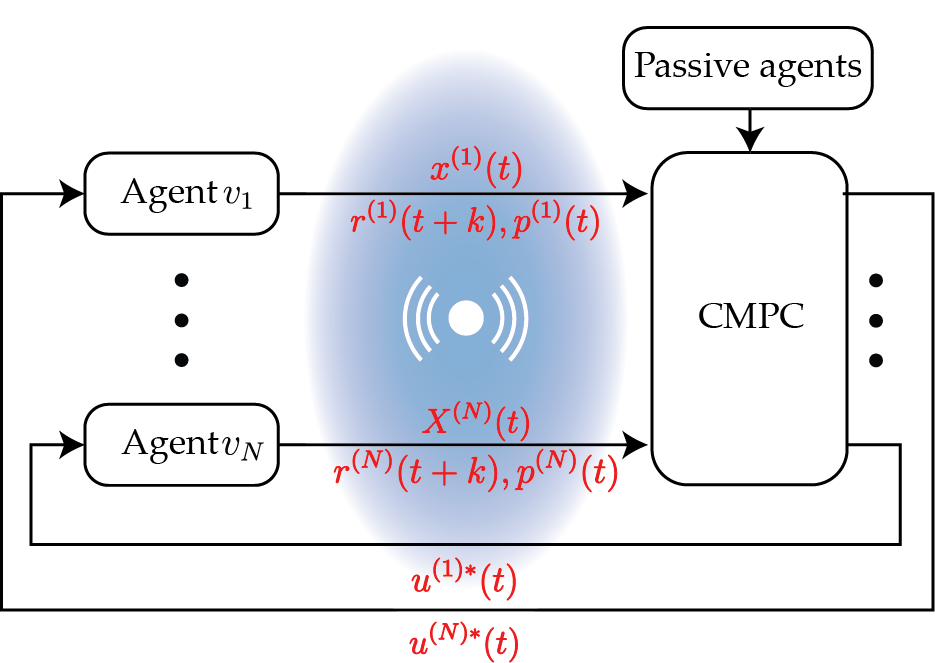
\includegraphics[width=0.6\textwidth]{Kap4/CMPC.png}
    \caption{Control architecture}
    \label{fig:CMPC}
\end{figure}


\subsection{Decentralized MPC}
\label{subsec:descentr}
In decentralized systems, the entire network relies on a single control node. However, as the network grows, the computation and synchronization of the agents become exponentially more difficult. However, suppose we decompose the whole network optimization problem into subproblems and rely on the communication between the neighbours. In that case, each subsystem will be able to obtain its own control input and achieve its goal even when some of the nodes are disconnected from the network. The architecture of the complete network can be seen in Fig.\ref{fig:DMPC}. This method is adopted from \cite{13t_distributed,32t_DMPC}.
% \subsubsection{Cooperative MPC}

\subsubsection{Neighbors $\mathcal{N}_i$}
Two or more vehicles are considered neighbors if:

\begin{align}
    \left\| p_i(t) - p_j(t) \right\| \le  \alpha d_{covered}
\end{align}

where $d_{covered} = v_i\ h$ means the distance that each vehicle covers in order to take into account other agents around it. $p_i(t)= \sqrt{x^2_i(t) + y^2_i(t)}$ and $\alpha \in (1,2)$. A pair of vehicles are considered "close neighbors" if:

\begin{align}
    \left| x_i(t+k) - x_j(t+k) \right| \le  d_{covered} \quad \& \quad \left| y_i(t+k) - y_j(t+k) \right| \lt \mu.
\end{align}

where $\mu$ means the road-width of a single lane.  
\\
\\
In the literature, the previous method is referred to as nonlinear distributed cooperative control \cite{12t_Dist_multiagent, 13t_distributed,32t_DMPC,51t_aveh2veh}. However, this method is not based on distributed optimization. Therefore, to avoid confusion, it will be called decentralized MPC (Dec. MPC).
\\
\\
All subsystems solve their optimization problem. Therefore, each vehicle $i \in \mathcal{V}$ must know the trajectories predicted by its neighbours $j \in \mathcal{N}_i$, which are considered optimal and obtained in the previous iteration. In the first step $t=0$, the Optimal control problem OCP has not been resolved; therefore it has to be initialized. This starts with choosing a feasible value for the estimated control variable $\hat{u}_i$

\subsubsection{Initialization of estimated control. }
At every step of time the instance $\tau$ in interval $[t, t+ H_p]$, The estimated control $\hat{u}_i$ for each vehicle is defined as:

\begin{align}
    \left\{ \begin{array}{cl}
\hat{u}_i(\tau, t) & = u^*_i(\tau;(t-1)) \text{  if }\tau \in [\tau \ ,\ (t-1) + H_p) \\
\hat{u}_i(\tau, t) & = 0, \text{ if } x_i(t) = r_i(H_p) \textbf{ or } \text{ if } \tau \in [(t-1)+H_p \ ,\  t+H_p] 
\end{array} \right.
\label{eq:416}
\end{align}


$u^*_i(\tau; (t-1))$  denotes the optimal solution to the OCP of the previous MPC iteration with initial state $x_i(t-1)$. However, sometimes for the first step $t_o$ the OCP has not been solved, and it is required to have an optimal solution already established. We propose the following algorithm where a solution to the problem is defined in the interval $[(t_0-1), (t_0-1) + H_p]$



\begin{algorithm}[H]
\caption{OCP initialization}\label{alg:ocp}
% \begin{algorithmic}
% \FOR $i \in \mathcal{V}$
% \FOR \forall {$i \in \mathcal{V}$} 
\If{$\tau \in (t_0 -1 )$}
        \For{ \forall $\tau \in [(t_0 -1), (t_0 -1)+H_p]$ \And $\mathcal{K} =+\infty$} 
        \State \text{solve \ref{eq:417}  with the initial state } $x_i(t_0 -1)$, $x_j(t_0 -1$ \And $\hat{u}_j(\tau ;x_j(t_0-1))=0$. 
        \EndFor
    \EndIf
% \end{algorithmic}
\end{algorithm}

The result obtained by the algorithm \ref{alg:ocp} is the optimal solution given the previously named initial conditions in the interval $[t_0, t_0 + H_p]$.
\\
\\
During each MPC iteration, the states and control signal obtained at $(t_o-1)$ over the interval $\tau \in [(t_0-1), (t_0-1) + H_p]$ are defined by $x_i^ *(\tau ; x_i(t_0 - 1))$ as current states and the control signal as $u_i^*(\tau ; x_i(t_0 - 1)$. $u_i^*$ is applied to each vehicle $i$ over time $[(t_0 - 1 ), (t_0 - 1 ) + H_p]$.
\\
\\
Again, the Decentralized Nonlinear MPC for Vehicle Collision Avoidance Problem use a nonlinear bicycle model \ref{eq:nonlinear_model} to represent the dynamics of the vehicles $i \in \mathcal{V}$ at time $t$ in the decentralized network: 

\newpage

\begin{multline}
    V^*_i(x(0 ), \hat{x}_j(\cdot), u_i(\cdot )) = \min_{x(\cdot ), u(\cdot )} \left ( \sum^{Hp-1}_{k=1} \ell_{x_{i}}(x_i(t+k),r_i(t+k)) + V_{if}(x_i(Hp)) + \right. \\
&\left.\sum^{Hu-1}_{i=1} \ell_{u_{i}} (u_i(t+k) ) + \sum_{j \in  \mathcal{N_{i,j} \neq i}} \sum^{H_p -1}_{k=1} \gamma \left\| L_{col}(\mu_{i,j}(x_i, \hat{x}_j)) \right\| ^{2} \right  ),
\end{multline}
\\
Subject to $(\forall _{i,j} \in \mathcal{N}_i ):$
\\
\begin{align}\label{eq:417} 
% \begin{matrix} 
& x_i(t+1+k)=f_i(x_i(t+k), u_i(t+k)), \quad & k=0, ..., H_p, \\ 
& \hat{x}_j(t+1+k) \in X_i, \quad & k=0, ... ,H_p, \\  
& x_i(t+k) \in \mathcal{X}_i, & k=1,...,H_p, \\ 
& u_i(t+H_p) \in \mathcal{U}_i, \quad  &k=0, ..., H_u - 1, \\ 
&\left\| x_i(t+k) - \hat{xx}_i(t+k) \right\| \le h^2 \mathcal{K}
% \end{matrix}
\label{eq:descentMPC}
\end{align}

\\
The objective function in the equation \ref{eq:descentMPC} is equivalent to the equation \ref{eq:centMPC}. However, many constraints have been modified for the decentralized controller. Each of them is explained in more detail below.

\begin{itemize}
    \item $L_{col}(\mu_{i,j}(x_i, \hat{x}_j)): \mathbb{R}^{n_i}\times \mathbb{R}^{n_j} \to \mathbb{R}$ describes the cost it would have on the OCP for vehicle $i$ to have a collision with vehicle $j \in \mathcal{N}_i$ :
    \begin{equation*}
        \sum_{j \in \mathcal{N}, j \neq i} \sum_{k+1}^{H_p -1 }\gamma \left\| L_{col}(\mu_{i,j}(t+k)) \right\|^2  \text{Where, } L_{col}(t) = \left\{ \begin{array}{cl}
\frac{1}{\left\| x_i(t) - x_j (t)\right\| -2D_i} & : \ \text{if  } j \in \mathcal{N}_i\\
0 & :\text{if } j \in \mathcal{N}_i
\end{array} \right. 
    \end{equation*}
    \item $f_j: \mathbb{R}^{n_j}\times \mathbb{R}^{m_j} \to \mathbb{R}^{n_j}$ describes the prediction model of the other vehicles $j$ in the neighborhood $\mathcal{N}_i$.
    \item $\hat{x}_j(t+k): \mathbb{R}^{n_j}$ represents the states that were communicated from the previous iteration of the MPC.
    \item $\left\| x_i(t+k) - \hat{x}_i (t+k)\right\| \le h^2 \mathcal{K}:\mathbb{R}^{n_i} \times \mathbb{R}^{n_j} \to \mathbb{R}$ denotes the compatibility of agent $i$ constraints with its previous results. Here, $h^2 \mathcal{k}$ is close to zero, meaning feasibility for each computed control input.
\end{itemize}

In the same way as in C-MPC, the OCP in \ref{eq:descentMPC} is solved with the Gurobi optimizer. 

% ///////////////////////////////////////////////////////////////////////////

% ///////////////////////////////////////////////////////////////////////////

\begin{figure}[H]
    \centering
    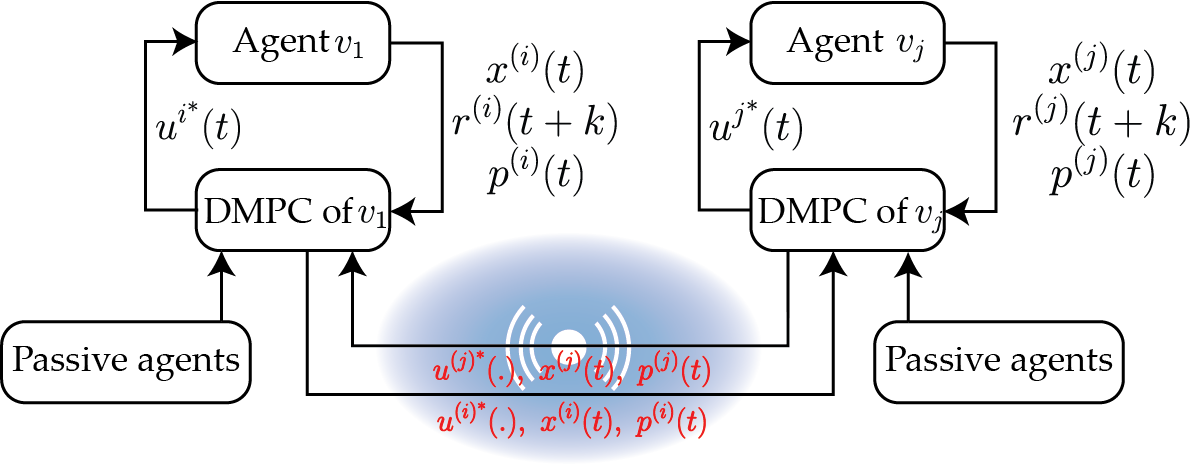
\includegraphics[width=0.8\textwidth]{Kap4/DMPC.png}
    \caption{Control architecture}
    \label{fig:DMPC}
\end{figure}

% \subsubsection{Potential Game}


% $$$$$$$$$$$$$$$$$$$$$$$$$$$
\subsection{Solution Method}

Solving a generalized Nash equilibrium problem is challenging even when only continuous variables are used. Our Optimization problem is a GNEP with mixed integer variables, and although it is used in both centralized and decentralized networks, its solution demands a large amount of computation. therefore, for \cite{18t_article} we use the Gauss-seidel method to calculate the $\epsilon$-MINE of the MVAD problem through iterations. This method solves the GNEP despite the mixed nature of \ref{eq:MPC_problem}
\\
\\
We will refer to the algorithmic step as an iteration to compute the solution and to the time step as a sample step of the decision variables. $x_i(k)$ denotes the decision vector of the agent $i$ at the k-th step of the algorithm. Moreover, the $x_i(t|k)$ as the k-th step at time t of the i-th agent in the solution algorithm. Finally, the cost variance will be $\Delta J_i(k)  := J_i(x_i(k)) - J_i(x_i^*(k))$, where $x^*_i(k) \in x^*_i(x_{-i}(k))$ will be the optimal decision vector of the i-th agent concerning its neighbours.


\subsubsection{Gauss-Seidel Algorithm}

We use a gauss seidel method of \cite{multivehicle} for solution of the problem \ref{eq:MPC_problem} we use a gauss seidel method of \cite{}. The algorithm follows a consecutive and ordered sequence to solve the optimization problem for each agent in the decentralized network and the entire network simultaneously in the centralized network. In the algorithm \ref{alg:centralize} the steps that the controller follows to compute the equilibrium of the GMIPG are detailed.






\begin{algorithm}[H]
\caption{Gauss-Seidel method for Centralized Networks}\label{alg:centralize}
% \begin{algorithmic}
\ForAll{ $i \in \mathcal{I}$} {
\State The controller choose a feasible state $x\in \hat{\mathcal{X}}_t$ for the whole network at time $t=0$ and set $k:=0$
    \While{$x(k)$ is not an $\epsilon$-MINE}{
    \State Load $x(t+1|k) $
    \ForAll{$i \in \mathcal{O}$}{
        \State $x_i (k+1) := \left\{ \begin{array}{cl} x_i^*(k) & \text{if  } \Delta J_i(k) \leq  \epsilon\\
    x_i(k) & \text{Otherwise} 
    \end{array} \right.$
        \State Load $x_i(t+1|k+1)$ to be use in the next step.
        }
    \EndFor
    }
    \State Set $k:=k+1$
    \End
    }
% \end{algorithmic}
\end{algorithm}




Given a pair of neighbouring agents $(j_1,j_2) \in \mathcal{I}^2$, we say that $j_1$ has a lower order if the distance $\sqrt{}$ of the agent $j_1$ is less than the distance of agent $j_2$.

thus, for each time step $t \in \mathcal{T}$ we define an ordered and closed set of neighbors. In the centralized network, the set of neighbours is complete and is always of the same size.



\begin{algorithm}[H]
\ForAll{ $i \in \mathcal{I}$} {
\State Each agent $i$ choose a feasible state $x(0) \in \hat{\mathcal{X}}_t$ and set $k:=0$
    \While{$x(k)$ is not an $\epsilon$-MINE}{
    \State Broadcast $x_i(t+1|k) $
    \ForAll{$i \in \mathcal{O}$}{
        \State $x_i (k+1) := \left\{ \begin{array}{cl} x_i^*(k) & \text{if} \Delta J_i(k) \leq  \epsilon\\
    x_i(k) & \text{Otherwise} 
    \end{array} \right.$
        \State Broadcast $x_i(t+1|k+1)$ to all $j \succ_t i$
        }
    \EndFor
    }
    \State Set $k:=k+1$
    \End
    }
% \end{algorithmic}
\caption{Gauss-Seidel method for Decentralized Networks}\label{alg:descentralize}
\end{algorithm}



In the decentralized network, the ordered neighbour group differs from the previous method. given a pair of vehicles $(i,j)$ the algorithm considers them neighbors if $d_{i,j} \leq D_covered$ ordering and selecting the closest ones. the algorithm \ref{alg:descentralize} gives an initial condition to each of the subsystems. then each subsystem shares its states and predicted trajectories to its neighbours $\mathcal{O}_t$, each controller with the information obtained from its neighbours and its current conditions calculates a solution to the problem \ref{eq:MPC_problem}. the last step is to share the new trajectories $x(t+1|k+1)$ to the neighbors.



\section{Mid-Level control}
 
 \begin{figure}[H]
\centering
    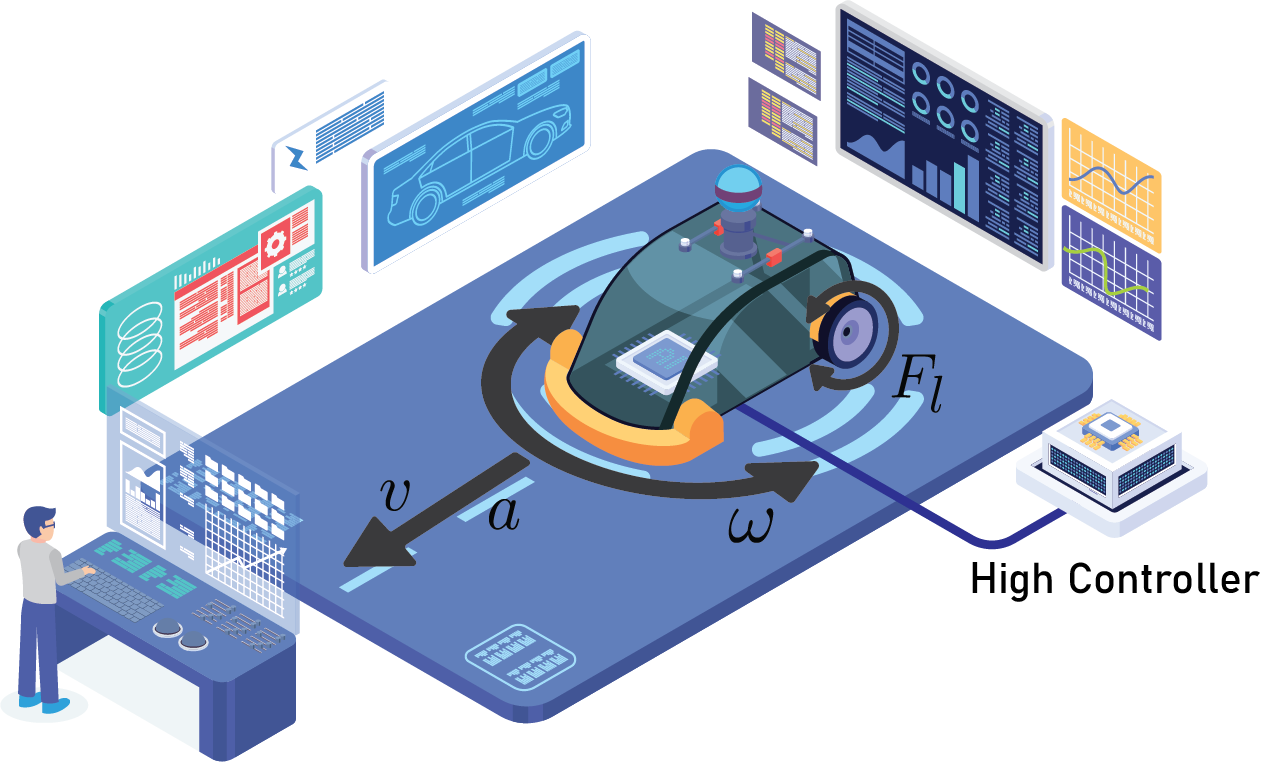
\includegraphics[width=0.55\textwidth]{Kap3/control_model.png}
    % \caption{Non-linear model of a differential robot.}
    % \label{non_linearmodel}
\end{figure}
 
A non-interconnected Model Predictive control was chosen for the Mid-Level controller. This method was chosen for its ease and robustness with nonlinear models. To set up this controller, we took into account the following features:
\begin{itemize}
    \item The mid-level controller will not have a connection with the other agents, only with the high and low-level controller of each vehicle.
    \item The reference trajectory is given as the predicted trajectories of the upper high-level controller.
    \item The result chosen by the mid-level controller is the linear speed $v$ and angular speed $\omega$ of the vehicle in its environment.
    \item The controller will have sensors that will detect if another obstacle, such as vehicles, people, or obstructions, is in the way.
\end{itemize}

Next, more detailed information about the mid-level controller will be given. We will not go deep into detail because the main contribution of this thesis is found in the high-level controller.

\subsection{Overview} 
 
The main goal of any MPC is to solve an optimization problem with some constraints by minimizing certain control variables. Let us introduces the cost function $J( x_p, y_p )$, which we wish to minimize, being $f(x,y)$ the nonlinear model of the section \ref{nonlinear_model} and $G(x,y)$ the constraint function, constrained within the range of $\left\{ g_{lb}, g_{ub} \right\}$.
 
\begin{align} 
\left\{\begin{matrix} 
\begin{aligned} 
\min_{v,\omega} \quad & J\left ( x_p, y_p \right )\\
\textrm{s.t.} \quad & l_{lb} \le f(x,y) \le l_{up}  \\
  &   g_{lb} \le G(x,y) \le g_{up}  
\end{aligned}
\end{matrix}\right.
\end{align}

Since the solution algorithm is discrete, it is necessary to discretize the nonlinear model. From \cite{mohamed} we discretize the equation \ref{nonlinear_model} as shown in the equation \ref{discrete_model}.

\begin{gather}
\left[ \begin{split}
\dot{x} \\ 
\dot{y} \\
\dot{\theta} 
\end{split} \right] = \left[ \begin{split}
 v \cos{\theta}\\ 
 v \sin{\theta} \\
\omega  
\end{split} \right]
\overset{\text{Euler Discretization}}{\longrightarrow}
\left[ \begin{split}
x(k+1) \\ 
y(k+1) \\
\theta(k+1) \\  
\end{split} \right]
=
\left[ \begin{split}
x(k) \\ 
y(k) \\
\theta(k) \\ 
\end{split} \right]
+ \Delta T
\left[ \begin{split}
 v(k) \cos{\theta}(k)\\ 
 v(k) \sin{\theta}(k) \\
\omega(k)  \\ 
\end{split} \right]
\label{discrete_model}
\end{gather}

The objective function as a standard MPC is defined as the square of the difference between the desired position and the vehicle's current position, adding the magnitude of the control variables. The first term punishes the error between the desired state and the current state. The second term seeks to use the least number of control units to reach the objective. The following equation describes the objective function to minimize:

\begin{equation}
    f(x,u)=\left\| x_o -x^{ref} \right\|^2_Q + \left\| u \right\|^2_R
\end{equation}

Finally, the set of constraints is composed of the discretized dynamic model $f(x(k),u(k))$, the constraints of the control variable $u(k) \forall k \in [0, H_p- 1]$ and the spatial constraints of the highway $x(k) \forall k \in [0, H_p]$

The objective OCP that each controller must solve in each iteration does not have dynamics or restrictions coupled with its other neighbours.

\begin{align}
    \left\{\begin{matrix} 
\begin{aligned} 
\min_{v,\omega} \quad & J\left ( x,u \right ) = \sum_{k=0}^{H_p-1} f(x(k),u(k))\\
\textrm{s.t.} \quad & x(k+1) = f(x(k),u(k)),  \\
  &   x(0) = x_0, \\
 & u(k) \in U, \forall k \in [0, H_p-1], \\
 & x(k) \in X, \forall k \in [0, H_p].
\end{aligned}
\end{matrix}\right.
\end{align}

In the implementation, the Python programming language was used together with the ARGroHBotS \cite{agrobots} test lab. The GUROBI library was used to be able to provide faster solutions when it was implemented in real-time.




% ///////////////////////////////////////////////
\section{Low-Level control}

\begin{figure}[H]
\centering
    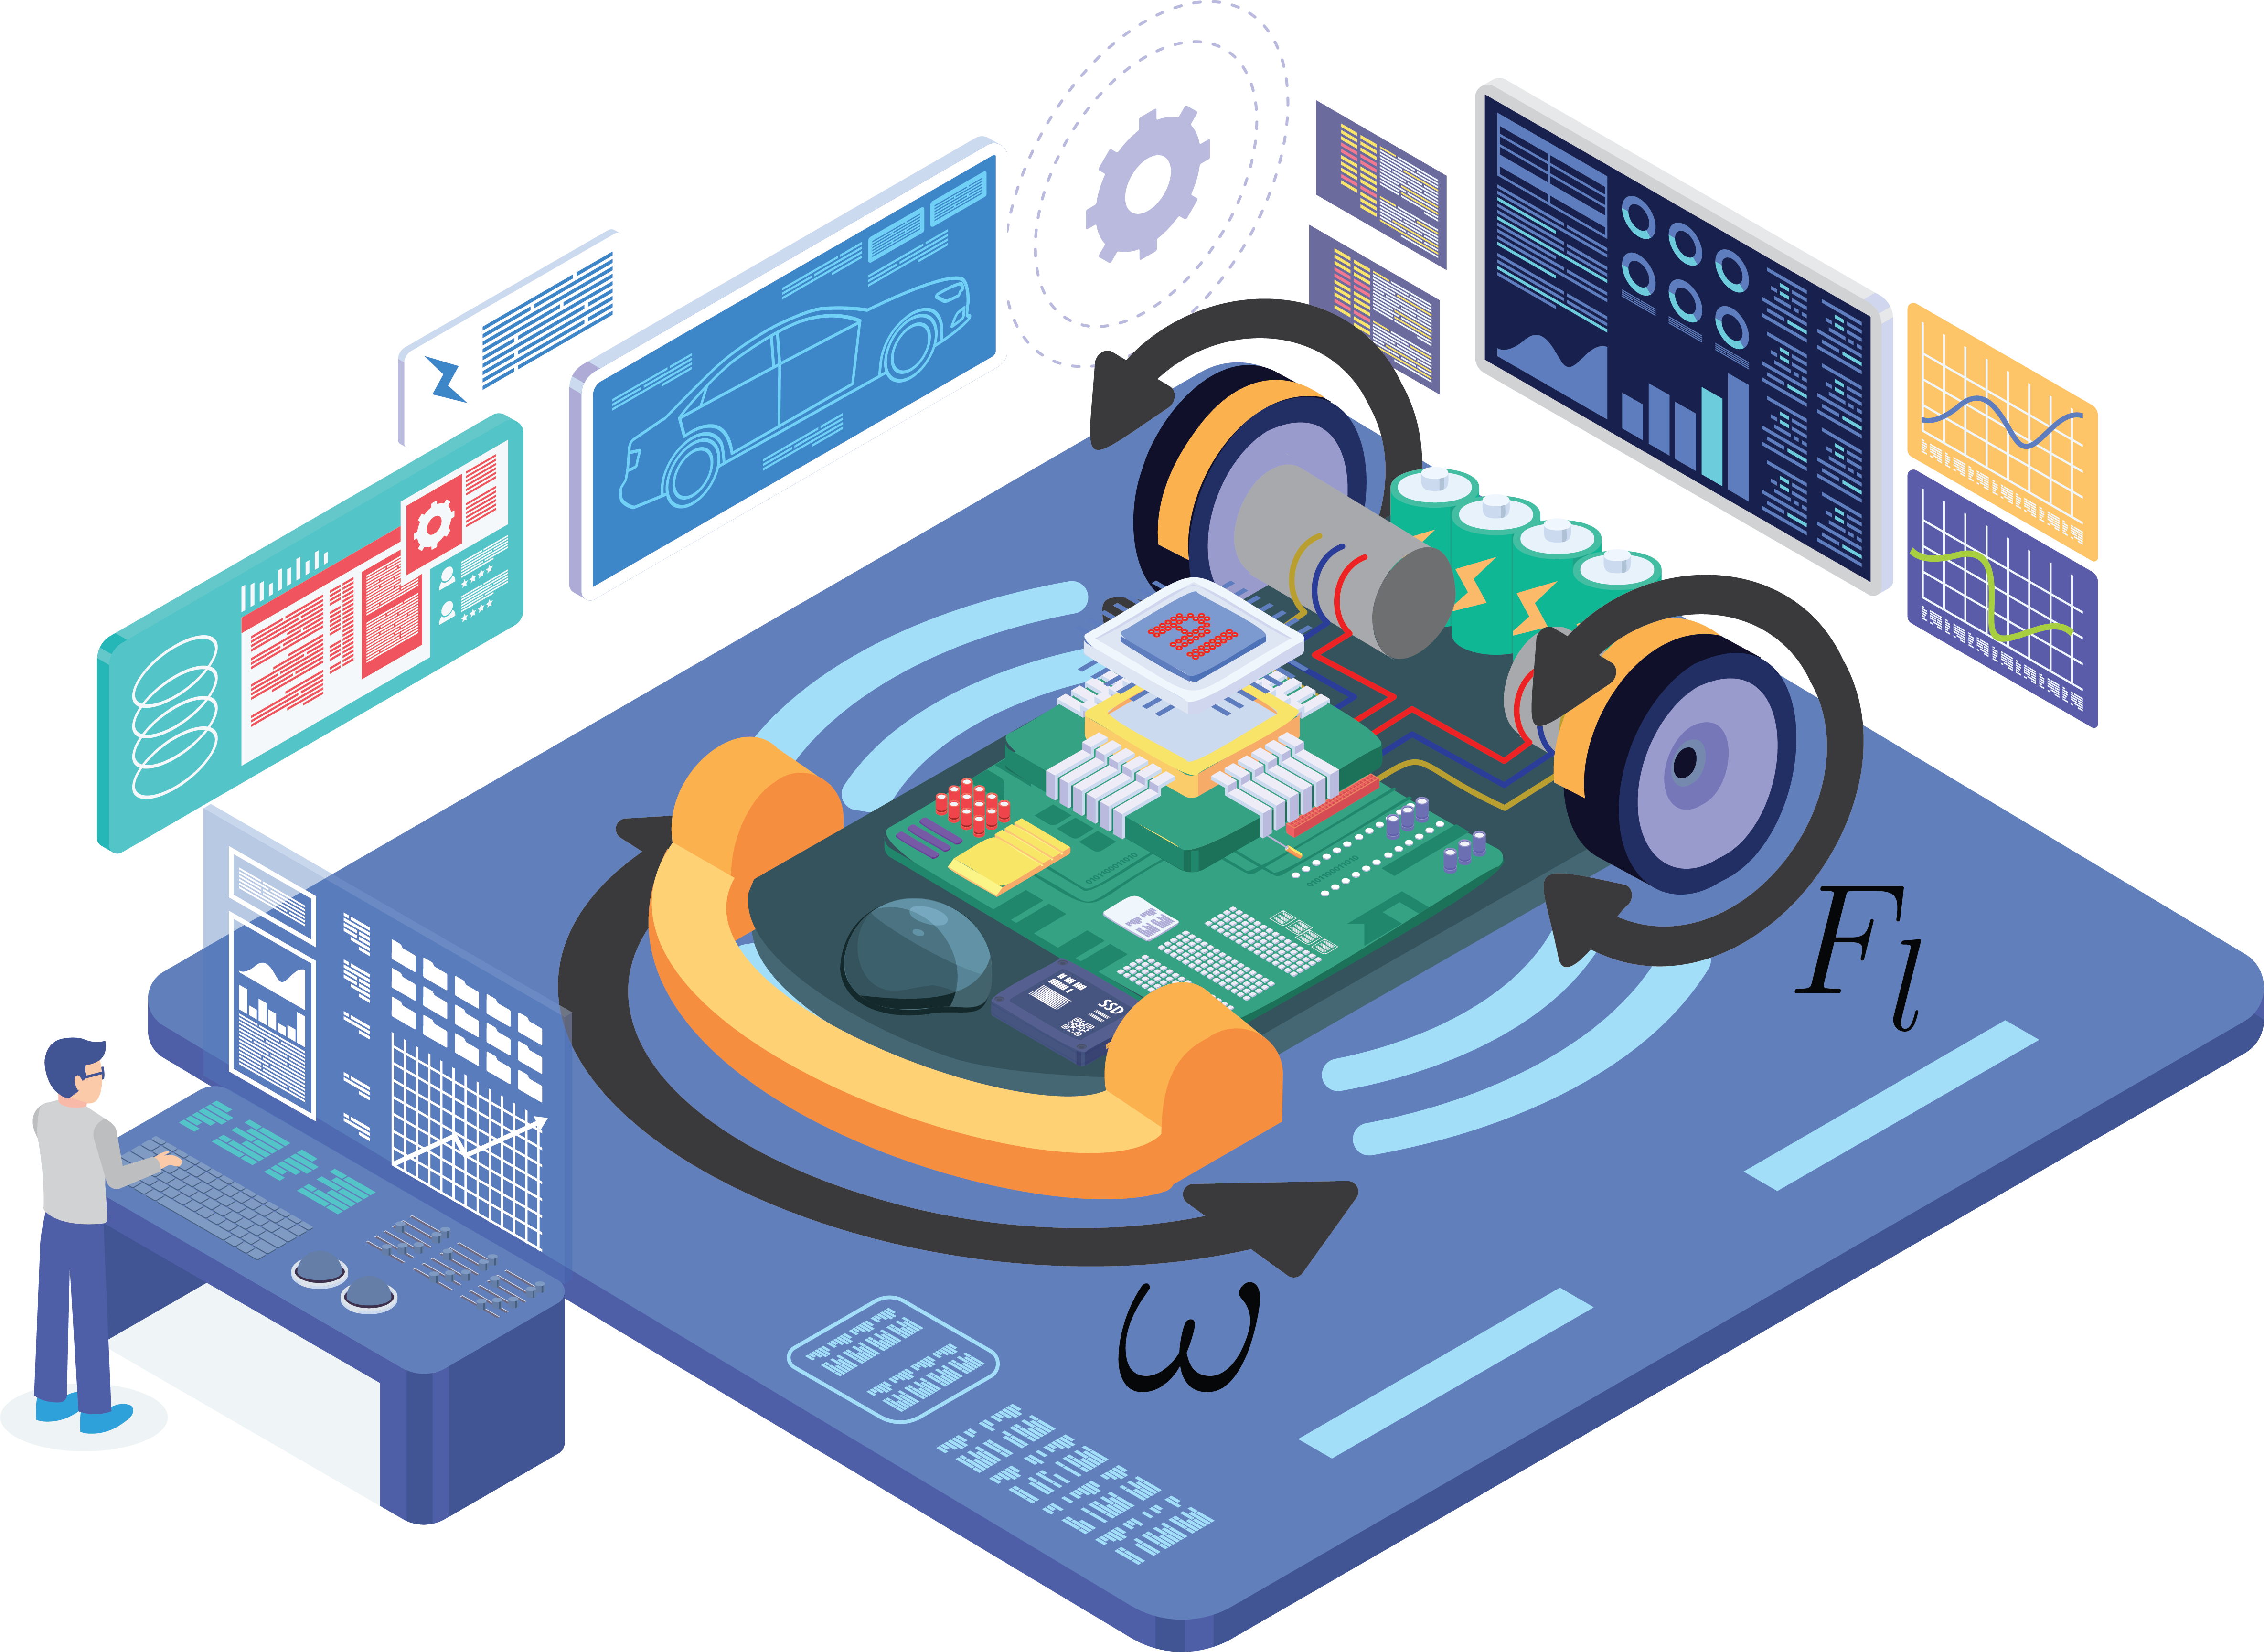
\includegraphics[width=0.55\textwidth]{Kap3/PID_model.png}
    % \caption{Non-linear model of a differential robot.}
    % \label{non_linearmodel}
\end{figure}



A proportional Integral Differential controller (PID) was implemented for the controller integrated into the robot. This was chosen for its ease, low computation level and easy adjustment. Each of the agents has a microchip \ref{processing} with a low level of processing, so it is necessary to have solution algorithms with low computational consumption. However, it is enough to give a sufficiently optimal solution to the problem. The controller receives the reference position delivered by the mid-level controller and transforms it into the angular velocity of each wheel.

\\
\\

We define the control signal as the solution to the following mathematical equation:

\begin{equation}
    u(t)= k_p e(t)+k_i \int_0^t e(\tau)\ d\tau + k_d \ \frac{d e(t)}{dt},
\end{equation}

where the proportional constant $K_p = 30$, the integral constant $k_i = 0.1$ and the differential constant $k_d = 1$.



 In Figure \ref{times}, each controller delivers a response at a different time. This is due to the complexity, high computational load and the level of communication each level handles. The simulation results will be discussed in the next chapter.

\begin{figure}[H]
\centering
    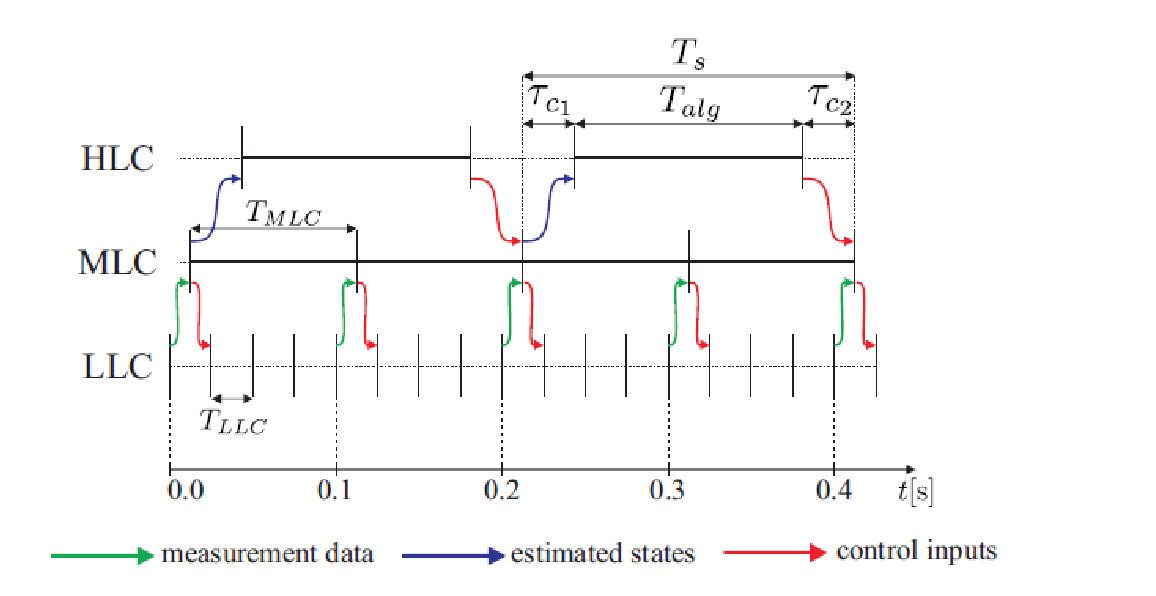
\includegraphics[width=0.7\textwidth]{Kap4/tiempos.png}
    \caption{Illustration of the interaction between the hierarchical levels.}
    \label{times}
\end{figure}